\begin{figure}[hb!]
\centering
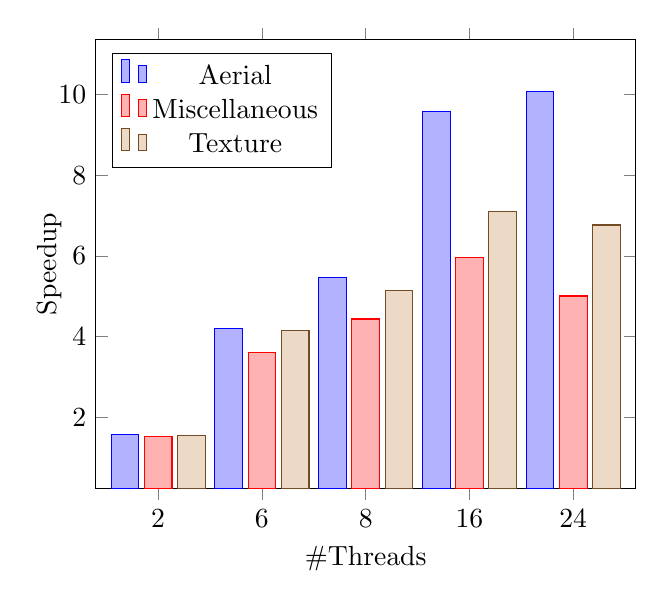
\begin{tikzpicture}
\begin{axis}[
ybar,
enlargelimits=0.15,
legend pos = north west,
xlabel=\#Threads,
ylabel=Speedup,
every axis y label/.style=
{at={(ticklabel cs:0.5)},rotate=90,anchor=center},
symbolic x coords={2,6,8,16,24},
xtick=data,
]
\addplot
coordinates {
(2,1.57)
(6,4.20)
(8,5.46)
(16,9.58)
(24,10.08)

};
\addplot
coordinates {
(2,1.53)
(6,3.60)
(8,4.44)
(16,5.96)
(24,5.01)
};
\addplot
coordinates {
(2,1.56)
(6,4.16)
(8,5.14)
(16,7.10)
(24,6.77)
};

\legend{Aerial,Miscellaneous,Texture}
\end{axis}
\end{tikzpicture}
\caption{Speedup for different images and different numbers of threads for
Aerial, Texture \& Miscellaneous data set}
\label{fig:bar}
\end{figure}
